\documentclass[12pt]{article}
\usepackage{amsmath}
\usepackage{array}
% \usepackage{gensymb}
\usepackage{geometry}
\usepackage{graphicx}
\usepackage{pgfplots}
\usepackage{siunitx}
\usepackage{wrapfig}

\title{Homework \#9}
\author{Donald Aingworth IV}
\date{October 16, 2024}

\pgfplotsset{width=8cm,compat=1.9}
\usepgfplotslibrary{external}
% \tikzexternalize

\begin{document}

\DeclareSIUnit{\mile}{mi}
\DeclareSIUnit{\gal}{gal}
\DeclareSIUnit{\foot}{ft}
\DeclareSIUnit{\h}{h}

% \maketitle

% \pagebreak
\section*{Problem 1}
A spring gun with k = 90.0 N/m is compressed by 5 cm. What is the exit speed of a 2.10-g projectile?

\subsection*{Solution}

\begin{align*}
    W   &= \int_{min}^{max} F(x)\ dx = \int_{-0.05}^{0} -kx\ dx = \left(-\frac{1}{2}kx^2\right)\vert_{-0.05}^{0} \\
        &= \frac{1}{2}k*0.05^2 = 45\unit{\newton/\meter} * 0.0025\unit{\meter^2} = 0.1 \unit{\joule}\\
    W   &=  \Delta K = K_f - K_i
\end{align*}
Since the spring on the block is unmoving at the start, then $v_i = 0$, so $K_i = \frac{1}{2}mv_i^2$ is also equal to zero. From there, we can determine the final kinetic energy and determine the velocity at the end.

\begin{align*}
    K_f &= W = 0.1\unit{\joule} = \frac{1}{2}mv_f^2\\
    \frac{2K_f}{m} &= v_f^2\\
    v_f &= \sqrt{\frac{2K_f}{m}} 
        = \sqrt{\frac{2*0.1\unit{\joule}}{0.0021\unit{\kilo\gram}}}
        = \sqrt{\frac{2*1000}{21}}\\
        &= \boxed{\frac{20\sqrt{105}}{21} \unit{\meter/\second} \approx 9.759 \unit{\meter/\second}}
\end{align*}

\pagebreak
\section*{Problem 2}
(a) The United States, with a population of $2.2 \times 10^8$ people, consumes $5 \times 10^{19}$ J per year. What is the per capita consumption in watts? (b) The sun's radiation provides the earth with 1000 \unit{\watt/\meter^2}. Assuming solar energy can be converted to electrical energy with a 20\% efficiency, how much area is needed to serve the energy needs of each U.S. citizen?

\subsection*{Solution}
\subsubsection*{Section (a)}
The power is determined by the work ($W$) divided by the time, with a watt being a joule divided by a second. The per capita value is determined by division by the number of humans ($c$). Assuming a year of 365 days, we can calculate the number of seconds per year ($t$) first.
\begin{align*}
    t   &=  1 \text{ years} * \frac{365\text{ days}}{1\text{ years}} 
                            * \frac{24\text{ hours}}{1\text{ days}}
                            * \frac{3600\unit{\second}}{1\text{ hours}}
        =   31536 \times 10^3 \unit{\second}\\
    P   &=  \frac{W}{t}
        =   \frac{5 \times 10^{19} \unit{\joule}}{(31536 \times 10^3 \unit{\second})}
        =   \frac{5 \times 10^{16}}{31536} \unit{\watt}\\
        &=  1.58549 \times 10^{12}\ \unit{\watt}\\
    P_{per\ captia}  &=  \frac{1.58549 \times 10^{12}}{2.2 \times 10^8} \unit{\watt}\\
        &=  \boxed{ 7206.77 \unit{\watt} }
\end{align*}

\subsubsection*{Section (b)}
Since there is only a 20\% efficiency, the usable numbers of watts per square meter would be $ Wa = 1000\ \unit{\watt/\meter^2}*\frac{20}{100} = 200\ \unit{\watt/\meter^2} $. We can divide the total power necessary per citizen (which we calculated in part (a)) to get the area necessary.
\begin{align*}
    A   &= \frac{P}{Wa}
        = \frac{ 7206.77 \unit{\watt} }{ 200\ \unit{\watt/\meter^2} }
        = \boxed{36.03 \unit{\meter^2}}
\end{align*}

\pagebreak
\section*{Problem 3}
A 0.595-kg object is released from a height of 3.60 m and lands on the ground. Find: (a) the work done by gravity; (b) the change in kinetic energy of the ball; (c) the speed just before it lands using energy methods. Ignore air resistance.

\subsection*{Solution}
\subsubsection*{Section (a)}
The object is released directly downward, so the angle with the vertical would be $ \phi = 90 \unit{\degree} = \frac{\pi}{2} $, so $\cos(\phi) = \cos(\frac{\pi}{2}) = 1$. This simplifies the formula from $W_g = mgd\cos(\phi)$ to $W_g = mgd$.
\begin{align*}
    W_g &=  mgd
        =   0.595\unit{\kilo\gram} * 9.81\unit{\meter/\second^2} * 3.60 \unit{\meter} 
        =   \boxed{21.01302\unit{\joule}}
\end{align*}

\subsubsection*{Section (b)}
The change in kinetic energy is equal to the work done by it. Since the object is in freefall, the only work done on it is the gravitational work.
\[ \Delta K = W_g = \boxed{21.01302\unit{\joule}} \]

\subsubsection*{Section (c)}
We can here use the formula for kinetic energy given the change in kinetic energy. The initial kinetic energy, since it starts from no velocity, is zero.
\[ \Delta K = K_f - K_i = K_f - 0 = K_f \]
\begin{align*}
    \Delta K    = K_f   &= \frac{1}{2}mv_f^2\\
    v_f^2   &=  \frac{2K_f}{m} = \frac{2*21.01302\unit{\joule}}{0.595\unit{\kilo\gram}} = 70.632 \unit{\meter^2/\second^2}\\
    v_f     &=  \sqrt{70.632 \unit{\meter^2/\second^2}} = \boxed{8.4043 \unit{\meter/\second}}
\end{align*}

\pagebreak
\section*{Problem 4}
\begin{wrapfigure}{r}{0.35\textwidth}
    \vspace{-30pt}
    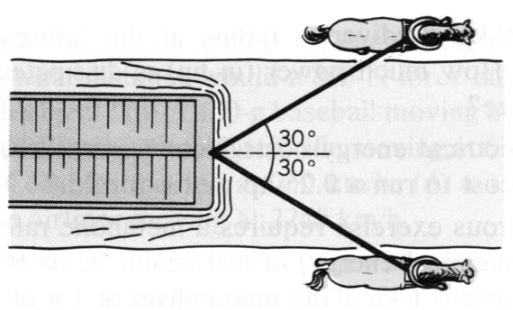
\includegraphics[width=0.35\textwidth]{graph_4.png} 
    % \label{fig:wrapfig}
\end{wrapfigure}
Two horses pull a barge along a canal at a steady 5.00 km/h, as shown in the figure. The tension in each rope is 420 N and each is at 30\unit{\degree} to the direction of motion. What is the horsepower provided by the horses?

\subsection*{Solution}
First, we convert units from km/h to m/s. 
\[ 5.00 \unit{\kilo\meter/\hour} * \frac{1000 \unit{\hour*\meter}}{3600 \unit{\kilo\meter*\second}} = \frac{25}{18} \unit{\meter/\second} \]

Now, we calculate from the tension the horizontal force exerted by each horse.
\[ F_x = T\cos(\phi) = 420\unit{\newton} * \cos(30\unit{\degree}) = 210*\sqrt{3}\unit{\newton} \]

Next, we multiply this force by the velocity of the horses to find the power of each individual horse, then multiply that by two to find the total horse power.
\begin{eqnarray*}
    P = F_x*v = (210*\sqrt{3}\unit{\newton}) * (\frac{25}{18} \unit{\meter/\second}) = \frac{875\sqrt{3}}{3} \unit{\watt}\\
    2*P = 2*\frac{875\sqrt{3}}{3} \unit{\watt} = \frac{1750\sqrt{3}}{3} \unit{\watt} = \boxed{1010.36 \unit{\watt}}
\end{eqnarray*}

% \pagebreak
% \section*{Problem 5}
% \begin{wrapfigure}{r}{0.35\textwidth}
%     \vspace{-30pt}
%     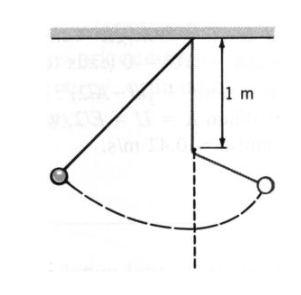
\includegraphics[width=0.35\textwidth]{graph_5.png} 
%     % \label{fig:wrapfig}
% \end{wrapfigure}


% \subsection*{Solution}

% \pagebreak
% \section*{Problem 6}
% \begin{wrapfigure}{r}{0.35\textwidth}
%     \vspace{-30pt}
%     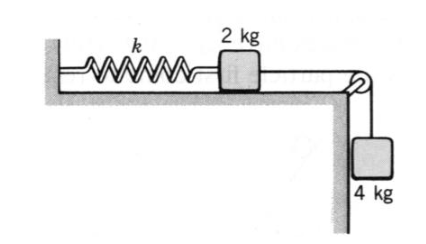
\includegraphics[width=0.35\textwidth]{graph_6.png} 
%     % \label{fig:wrapfig}
% \end{wrapfigure}


% \subsection*{Solution}

% \pagebreak
% \section*{Problem 7}
% \begin{wrapfigure}{r}{0.35\textwidth}
%     \vspace{-30pt}
%     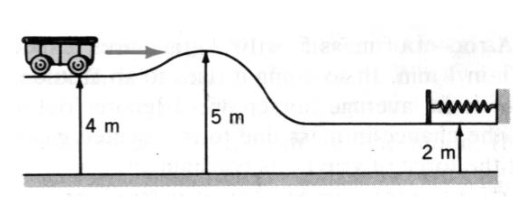
\includegraphics[width=0.35\textwidth]{graph_7.png} 
%     % \label{fig:wrapfig}
% \end{wrapfigure}


% \subsection*{Solution}

% \pagebreak
% \section*{Problem 8}


% \subsection*{Solution}


\end{document}